\section*{Problem J - Jumlah Opat}
\addcontentsline{toc}{section}{Problem J - Jumlah Opat}
\textit{Author: Jauhar Wibisono}
\\
\textit{Expected Difficulty: Medium}

Salah satu solusi untuk soal ini adalah algoritma \textit{Monte Carlo}. Apabila dipilih sebuah \textit{connected subgraph} secara acak, peluang jumlah nilai \textit{node}-nya habis dibagi 4 adalah $1/4$. Dengan kata lain, nilai harapan dari banyak percobaan memilih \textit{connected subgraph} sampai didapatkan \textit{connected subgraph} dengan jumlah nilai habis dibagi 4 adalah 4. Jadi, kita dapat mencoba berbagai \textit{connected subgraph} sampai solusi ditemukan atau sampai kita yakin bahwa tidak terdapat solusi pada graf yang diberikan.

Perlu diperhatikan bahwa \textit{tree} yang tidak memiliki \textit{connected subgraph} dengan jumlah nilai habis dibagi 4 mudah dibuat, contohnya seperti berikut.
\begin{center}
	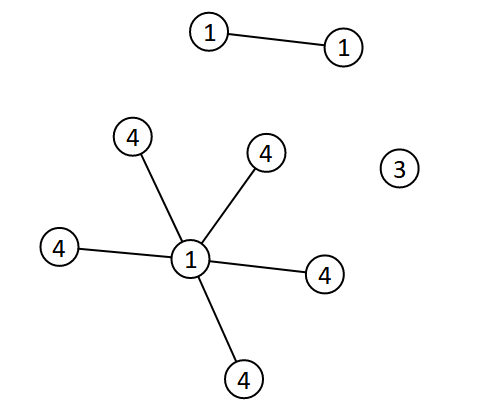
\includegraphics{arkavidia-2021-qual-jumlah-opat/impossible.png}
\end{center}
Jadi percobaan harus dilakukan secara merata untuk semua \textit{tree} agar \textit{tree} yang memiliki \textit{connected subgraph} dengan jumlah nilai habis dibagi 4 tidak terlewat.

Kode Solusi: \url{https://ideone.com/R5d1dV} (solusi random), \url{https://ideone.com/kDxhNV} (solusi DP)

Kompleksitas Waktu: $O(N)$

Catatan Panitia:

Tree terbesar yang hanya memiliki satu solusi yang ditemukan penulis soal memiliki 7 node, bisakah Anda mencari tree yang lebih besar?